\subsubsection{Subtree Mutation}
\label{sec:keen:op:mut:subtree}
    One key technique among mutation operators in GP is the Subtree Mutation. It serves to adjust the genetic structure 
    of program trees.

    \begin{definition}[Subtree Mutation]
        The \textit{subtree mutation} operator functions by picking a node from a program tree and replacing the subtree 
        from that node with a new one. This method maintains the overall structure of the program but adds new genetic 
        elements, potentially improving the program's performance.
    
        The mathematical representation of this operation is:
    
        \begin{equation}
            M_{subtree}: \mathbb{P} \times [0,\, 1] \times [0,\, 1] \times [0,\, 1] \rightarrow \mathbb{P};\;
            (P,\, \mu_\textbf{i},\, \mu_\textbf{c},\, \mu_\textbf{g}) 
                \mapsto M_{subtree}(P,\, \mu_\textbf{i},\, \mu_\textbf{c},\, \mu_\textbf{g})
        \end{equation}
    
        Explaining the parameters:
    
        \begin{itemize}
            \item \(P\): The population of program trees.
            \item \(\mu_\textbf{i}\): The chance of a tree undergoing mutation.
            \item \(\mu_\textbf{c}\): The likelihood of choosing a chromosome for mutation.
            \item \(\mu_\textbf{g}\): The probability of selecting a gene for mutation.
        \end{itemize}
    \end{definition}

    In the \textit{Keen} framework, the Subtree Mutation process happens like this:

    \begin{code}{
        Explaining Subtree Mutation in \textit{Keen}
    }{label=lst:keen:op:mut:subtree}{kotlin}
        val targetNode = choose random node from program tree
        val newSubtree = create a new subtree
        val mutatedTree = replace targetNode's subtree in program tree with newSubtree
    \end{code}

    In essence, the Subtree Mutation in \textit{Keen} adds new genetic components without heavily changing the main 
    structure of the tree.

    \begin{remark}
        The Subtree Mutation operator is effective for introducing substantial genetic alterations. However, it's 
        crucial to ensure that the newly generated subtrees are relevant and appropriate for the specific problem at 
        hand. Without careful consideration, there's a risk of creating trees that are either semantically irrelevant or 
        overly complex.

        In \textit{Keen}, this concern is addressed by employing specific subtree generation methods, as detailed in \vref{sec:keen:gp:primitives:gen}.
    \end{remark}

    For a visual representation of the Subtree Mutation process, see \vref{fig:keen:op:mut:subtree}.

    \begin{figure}[ht!]
        \centering
        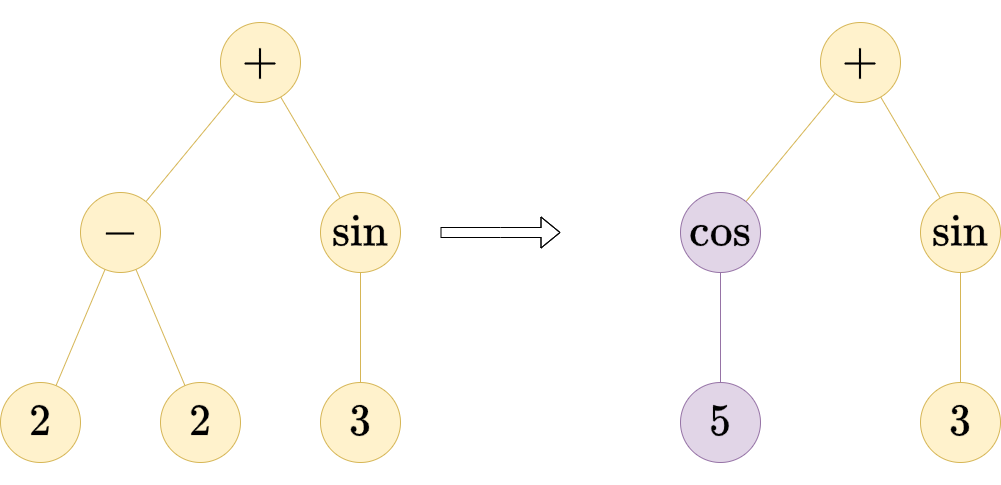
\includegraphics[width=0.5\textwidth]{img/keen/STM.png}
        \caption{
            A visual guide to the Subtree Mutation process. The operator picks a node and replaces its attached subtree 
            with a new one, giving a changed but still recognizable program tree.
        }
        \label{fig:keen:op:mut:subtree}
    \end{figure}
